
%% bare_conf.tex
%% V1.4b
%% 2015/08/26
%% by Michael Shell
%% See:
%% http://www.michaelshell.org/
%% for current contact information.
%%
%% This is a skeleton file demonstrating the use of IEEEtran.cls
%% (requires IEEEtran.cls version 1.8b or later) with an IEEE
%% conference paper.
%%
%% Support sites:
%% http://www.michaelshell.org/tex/ieeetran/
%% http://www.ctan.org/pkg/ieeetran
%% and
%% http://www.ieee.org/

%%*************************************************************************
%% Legal Notice:
%% This code is offered as-is without any warranty either expressed or
%% implied; without even the implied warranty of MERCHANTABILITY or
%% FITNESS FOR A PARTICULAR PURPOSE!
%% User assumes all risk.
%% In no event shall the IEEE or any contributor to this code be liable for
%% any damages or losses, including, but not limited to, incidental,
%% consequential, or any other damages, resulting from the use or misuse
%% of any information contained here.
%%
%% All comments are the opinions of their respective authors and are not
%% necessarily endorsed by the IEEE.
%%
%% This work is distributed under the LaTeX Project Public License (LPPL)
%% ( http://www.latex-project.org/ ) version 1.3, and may be freely used,
%% distributed and modified. A copy of the LPPL, version 1.3, is included
%% in the base LaTeX documentation of all distributions of LaTeX released
%% 2003/12/01 or later.
%% Retain all contribution notices and credits.
%% ** Modified files should be clearly indicated as such, including  **
%% ** renaming them and changing author support contact information. **
%%*************************************************************************


% *** Authors should verify (and, if needed, correct) their LaTeX system  ***
% *** with the testflow diagnostic prior to trusting their LaTeX platform ***
% *** with production work. The IEEE's font choices and paper sizes can   ***
% *** trigger bugs that do not appear when using other class files.       ***                          ***
% The testflow support page is at:
% http://www.michaelshell.org/tex/testflow/



\documentclass[conference]{IEEEtran}
% Some Computer Society conferences also require the compsoc mode option,
% but others use the standard conference format.
%
% If IEEEtran.cls has not been installed into the LaTeX system files,
% manually specify the path to it like:
% \documentclass[conference]{../sty/IEEEtran}


% customized definitions:
\def\lycoris{\textsc{Lycoris }}%

% Some very useful LaTeX packages include:
% (uncomment the ones you want to load)


% *** MISC UTILITY PACKAGES ***
%
%\usepackage{ifpdf}
% Heiko Oberdiek's ifpdf.sty is very useful if you need conditional
% compilation based on whether the output is pdf or dvi.
% usage:
% \ifpdf
%   % pdf code
% \else
%   % dvi code
% \fi
% The latest version of ifpdf.sty can be obtained from:
% http://www.ctan.org/pkg/ifpdf
% Also, note that IEEEtran.cls V1.7 and later provides a builtin
% \ifCLASSINFOpdf conditional that works the same way.
% When switching from latex to pdflatex and vice-versa, the compiler may
% have to be run twice to clear warning/error messages.






% *** CITATION PACKAGES ***
%
\usepackage{cite}
% cite.sty was written by Donald Arseneau
% V1.6 and later of IEEEtran pre-defines the format of the cite.sty package
% \cite{} output to follow that of the IEEE. Loading the cite package will
% result in citation numbers being automatically sorted and properly
% "compressed/ranged". e.g., [1], [9], [2], [7], [5], [6] without using
% cite.sty will become [1], [2], [5]--[7], [9] using cite.sty. cite.sty's
% \cite will automatically add leading space, if needed. Use cite.sty's
% noadjust option (cite.sty V3.8 and later) if you want to turn this off
% such as if a citation ever needs to be enclosed in parenthesis.
% cite.sty is already installed on most LaTeX systems. Be sure and use
% version 5.0 (2009-03-20) and later if using hyperref.sty.
% The latest version can be obtained at:
% http://www.ctan.org/pkg/cite
% The documentation is contained in the cite.sty file itself.






% *** GRAPHICS RELATED PACKAGES ***
%
\ifCLASSINFOpdf
  \usepackage[pdftex]{graphicx}
  % declare the path(s) where your graphic files are
  % \graphicspath{{../pdf/}{../jpeg/}}
  % and their extensions so you won't have to specify these with
  % every instance of \includegraphics
  % \DeclareGraphicsExtensions{.pdf,.jpeg,.png}
\else
  % or other class option (dvipsone, dvipdf, if not using dvips). graphicx
  % will default to the driver specified in the system graphics.cfg if no
  % driver is specified.
  % \usepackage[dvips]{graphicx}
  % declare the path(s) where your graphic files are
  % \graphicspath{{../eps/}}
  % and their extensions so you won't have to specify these with
  % every instance of \includegraphics
  % \DeclareGraphicsExtensions{.eps}
\fi
% graphicx was written by David Carlisle and Sebastian Rahtz. It is
% required if you want graphics, photos, etc. graphicx.sty is already
% installed on most LaTeX systems. The latest version and documentation
% can be obtained at:
% http://www.ctan.org/pkg/graphicx
% Another good source of documentation is "Using Imported Graphics in
% LaTeX2e" by Keith Reckdahl which can be found at:
% http://www.ctan.org/pkg/epslatex
%
% latex, and pdflatex in dvi mode, support graphics in encapsulated
% postscript (.eps) format. pdflatex in pdf mode supports graphics
% in .pdf, .jpeg, .png and .mps (metapost) formats. Users should ensure
% that all non-photo figures use a vector format (.eps, .pdf, .mps) and
% not a bitmapped formats (.jpeg, .png). The IEEE frowns on bitmapped formats
% which can result in "jaggedy"/blurry rendering of lines and letters as
% well as large increases in file sizes.
%
% You can find documentation about the pdfTeX application at:
% http://www.tug.org/applications/pdftex





% *** MATH PACKAGES ***
%
\usepackage{amsmath}
\usepackage{siunitx}

% A popular package from the American Mathematical Society that provides
% many useful and powerful commands for dealing with mathematics.
%
% Note that the amsmath package sets \interdisplaylinepenalty to 10000
% thus preventing page breaks from occurring within multiline equations. Use:
%\interdisplaylinepenalty=2500
% after loading amsmath to restore such page breaks as IEEEtran.cls normally
% does. amsmath.sty is already installed on most LaTeX systems. The latest
% version and documentation can be obtained at:
% http://www.ctan.org/pkg/amsmath





% *** SPECIALIZED LIST PACKAGES ***
%
%\usepackage{algorithmic}
% algorithmic.sty was written by Peter Williams and Rogerio Brito.
% This package provides an algorithmic environment fo describing algorithms.
% You can use the algorithmic environment in-text or within a figure
% environment to provide for a floating algorithm. Do NOT use the algorithm
% floating environment provided by algorithm.sty (by the same authors) or
% algorithm2e.sty (by Christophe Fiorio) as the IEEE does not use dedicated
% algorithm float types and packages that provide these will not provide
% correct IEEE style captions. The latest version and documentation of
% algorithmic.sty can be obtained at:
% http://www.ctan.org/pkg/algorithms
% Also of interest may be the (relatively newer and more customizable)
% algorithmicx.sty package by Szasz Janos:
% http://www.ctan.org/pkg/algorithmicx




% *** ALIGNMENT PACKAGES ***
%
%\usepackage{array}
% Frank Mittelbach's and David Carlisle's array.sty patches and improves
% the standard LaTeX2e array and tabular environments to provide better
% appearance and additional user controls. As the default LaTeX2e table
% generation code is lacking to the point of almost being broken with
% respect to the quality of the end results, all users are strongly
% advised to use an enhanced (at the very least that provided by array.sty)
% set of table tools. array.sty is already installed on most systems. The
% latest version and documentation can be obtained at:
% http://www.ctan.org/pkg/array


% IEEEtran contains the IEEEeqnarray family of commands that can be used to
% generate multiline equations as well as matrices, tables, etc., of high
% quality.




% *** SUBFIGURE PACKAGES ***
%\ifCLASSOPTIONcompsoc
%  \usepackage[caption=false,font=normalsize,labelfont=sf,textfont=sf]{subfig}
%\else
%  \usepackage[caption=false,font=footnotesize]{subfig}
%\fi
% subfig.sty, written by Steven Douglas Cochran, is the modern replacement
% for subfigure.sty, the latter of which is no longer maintained and is
% incompatible with some LaTeX packages including fixltx2e. However,
% subfig.sty requires and automatically loads Axel Sommerfeldt's caption.sty
% which will override IEEEtran.cls' handling of captions and this will result
% in non-IEEE style figure/table captions. To prevent this problem, be sure
% and invoke subfig.sty's "caption=false" package option (available since
% subfig.sty version 1.3, 2005/06/28) as this is will preserve IEEEtran.cls
% handling of captions.
% Note that the Computer Society format requires a larger sans serif font
% than the serif footnote size font used in traditional IEEE formatting
% and thus the need to invoke different subfig.sty package options depending
% on whether compsoc mode has been enabled.
%
% The latest version and documentation of subfig.sty can be obtained at:
% http://www.ctan.org/pkg/subfig




% *** FLOAT PACKAGES ***
%
%\usepackage{fixltx2e}
% fixltx2e, the successor to the earlier fix2col.sty, was written by
% Frank Mittelbach and David Carlisle. This package corrects a few problems
% in the LaTeX2e kernel, the most notable of which is that in current
% LaTeX2e releases, the ordering of single and double column floats is not
% guaranteed to be preserved. Thus, an unpatched LaTeX2e can allow a
% single column figure to be placed prior to an earlier double column
% figure.
% Be aware that LaTeX2e kernels dated 2015 and later have fixltx2e.sty's
% corrections already built into the system in which case a warning will
% be issued if an attempt is made to load fixltx2e.sty as it is no longer
% needed.
% The latest version and documentation can be found at:
% http://www.ctan.org/pkg/fixltx2e


%\usepackage{stfloats}
% stfloats.sty was written by Sigitas Tolusis. This package gives LaTeX2e
% the ability to do double column floats at the bottom of the page as well
% as the top. (e.g., "\begin{figure*}[!b]" is not normally possible in
% LaTeX2e). It also provides a command:
%\fnbelowfloat
% to enable the placement of footnotes below bottom floats (the standard
% LaTeX2e kernel puts them above bottom floats). This is an invasive package
% which rewrites many portions of the LaTeX2e float routines. It may not work
% with other packages that modify the LaTeX2e float routines. The latest
% version and documentation can be obtained at:
% http://www.ctan.org/pkg/stfloats
% Do not use the stfloats baselinefloat ability as the IEEE does not allow
% \baselineskip to stretch. Authors submitting work to the IEEE should note
% that the IEEE rarely uses double column equations and that authors should try
% to avoid such use. Do not be tempted to use the cuted.sty or midfloat.sty
% packages (also by Sigitas Tolusis) as the IEEE does not format its papers in
% such ways.
% Do not attempt to use stfloats with fixltx2e as they are incompatible.
% Instead, use Morten Hogholm'a dblfloatfix which combines the features
% of both fixltx2e and stfloats:
%
% \usepackage{dblfloatfix}
% The latest version can be found at:
% http://www.ctan.org/pkg/dblfloatfix




% *** PDF, URL AND HYPERLINK PACKAGES ***
%
\usepackage{url}
% url.sty was written by Donald Arseneau. It provides better support for
% handling and breaking URLs. url.sty is already installed on most LaTeX
% systems. The latest version and documentation can be obtained at:
% http://www.ctan.org/pkg/url
% Basically, \url{my_url_here}.




% *** Do not adjust lengths that control margins, column widths, etc. ***
% *** Do not use packages that alter fonts (such as pslatex).         ***
% There should be no need to do such things with IEEEtran.cls V1.6 and later.
% (Unless specifically asked to do so by the journal or conference you plan
% to submit to, of course. )


% correct bad hyphenation here
\hyphenation{op-tical net-works semi-conduc-tor}


\begin{document}
%
% paper title
% Titles are generally capitalized except for words such as a, an, and, as,
% at, but, by, for, in, nor, of, on, or, the, to and up, which are usually
% not capitalized unless they are the first or last word of the title.
% Linebreaks \\ can be used within to get better formatting as desired.
% Do not put math or special symbols in the title.
\title{{\sc Lycoris}{: A large area beam telescope based on hybrid-less strip silicon sensors}}


% author names and affiliations
% use a multiple column layout for up to three different
% affiliations
% \author{\IEEEauthorblockN{Michael Shell}
% \IEEEauthorblockA{School of Electrical and\\Computer Engineering\\
% Georgia Institute of Technology\\
% Atlanta, Georgia 30332--0250\\
% Email: http://www.michaelshell.org/contact.html}
% \and
% \IEEEauthorblockN{Homer Simpson}
% \IEEEauthorblockA{Twentieth Century Fox\\
% Springfield, USA\\
% Email: homer@thesimpsons.com}
% \and
% \IEEEauthorblockN{James Kirk\\ and Montgomery Scott}
% \IEEEauthorblockA{Starfleet Academy\\
% San Francisco, California 96678--2391\\
% Telephone: (800) 555--1212\\
% Fax: (888) 555--1212}}

% conference papers do not typically use \thanks and this command
% is locked out in conference mode. If really needed, such as for
% the acknowledgment of grants, issue a \IEEEoverridecommandlockouts
% after \documentclass

% for over three affiliations, or if they all won't fit within the width
% of the page, use this alternative format:
%
\author{
\IEEEauthorblockN{
Martin Breidenbach\IEEEauthorrefmark{2},
Dietrich R. Freytag\IEEEauthorrefmark{2},
Uwe Kraemer\IEEEauthorrefmark{1},
Benjamin A. Reese\IEEEauthorrefmark{2},
Sebastiaan Roelofs\IEEEauthorrefmark{1}\IEEEauthorrefmark{3},\\
Marcel Stanitzki\IEEEauthorrefmark{1} and
Mengqing Wu\IEEEauthorrefmark{1}
}

\IEEEauthorblockA{\IEEEauthorrefmark{1}Deutsches Elektronen-Synchrotron DESY, Notkestr. 85, 22607 Hamburg, Germany}
\IEEEauthorblockA{\IEEEauthorrefmark{2}Stanford Linear Accelerator Center SLAC, 2575 Sand Hill Road, Menlo Park, CA 94025 USA}
\IEEEauthorblockA{\IEEEauthorrefmark{3}The Hague University of Applied Sciences, Rotterdamseweg 137, 2628 AL Delft, The Netherlands}
}
% use for special paper notices
%\IEEEspecialpapernotice{(Invited Paper)}




% make the title area
\maketitle

% As a general rule, do not put math, special symbols or citations
% in the abstract
\begin{abstract}

A new Large area x-Y COverage Readout Integrated Strip telescope (\lycoris) is being constructed
as an improvement of the DESY test beam infrastructure within the Horizon2020 AIDA-2020 project~\cite{aida2020}.
The \lycoris telescope consists of six layers of \SI{25}{\micro\metre} pitch strip Si sensor readout by two bump-bonded ASICs (KPiX),
running at a timing resolution as multiples of \SI{80}{\nano\second};
its active area is designed to be $10\times$\SI{10}{\square\centi\metre}, extendable to $10\times$\SI{20}{\square\centi\metre}.
It can run either standalone or be mounted inside a \SI{1}{\tesla} solenoid magnet,
providing a spatial resolution better than \SI{10}{\micro\metre} along the bending direction,
and a resolution better than \SI{1}{\milli\metre} along the magnetic field.
The full readout system was tested with a hexagonal pixel sensor designed for the SiD ECAL in the lab with a $^{90}$Sr source,
and later tested in the electron beam at DESY in May and October 2017. The first assembled modules with the final strip were tested in spring 2018.
First results of the \lycoris prototype will be presented with a comparison to simulation,
besides, the characterization of sensor and readout system are also included.

\end{abstract}

% no keywords




% For peer review papers, you can put extra information on the cover
% page as needed:
% \ifCLASSOPTIONpeerreview
% \begin{center} \bfseries EDICS Category: 3-BBND \end{center}
% \fi
%
% For peerreview papers, this IEEEtran command inserts a page break and
% creates the second title. It will be ignored for other modes.
%\IEEEpeerreviewmaketitle

\section{Introduction}
% no \IEEEPARstart

The DESY II Test Beam Facility\cite{desytbf}
provides $e^-/e^+$ beams with energies from 1 to \SI{6}{\GeV} up to \SI{1}{\MHz}
%converted from bremsstrahlung beams from carbon fibre targets in the electron-positron synchrotron DESY II,
with three test beam lines (TB21, TB22 and TB24).
The beam lines TB21 and TB22 are both equipped with a EUDET-type beam telescope~\cite{eudet}
with an active area of around $1\times$\SI{2}{\square\centi\metre},
which is based on a fine pitch \uppercase{mimosa}~26 monolithic sensor with an event readout frame of \SI{115.2}{\micro\second};
the beam line TB24 is equipped with a \SI{1}{\tesla} solenoid, the PCMAG, at a diametre of $\sim$\SI{85}{\centi\metre} with its wall of $\sim20X_0$,
inside which both the EUDET-type telescope and the Device Under Test (DUT) can be inserted.
The EUDET-type beam telescopes at DESY are proven to meet user demands very well and thus in a high ($\sim$70\%) demand,
however, its active area is limited for momentum measurements for users in the PCMAG or for users requiring a larger tracker coverage.
Therefore, a new telescope is in need to provide a spatial resolution better than \SI{10}{\micro\metre} along the bending direction,
and a resolution better than \SI{1}{\milli\metre} along the magnetic field,
with a large active area of $10\times$10/\SI{20}{\square\centi\metre},
to cover 90\% to 96\% of the incoming particles with energies from 1 to \SI{6}{\GeV} considering momentum smearing after the magnet wall.

The \SI{320}{\micro\metre} thick, \SI{10}{cm} long, \SI{10}{cm} wide SiD micro-strip sensor has a sense/readout pitch of $25/$\SI{50}{\micro\metre},
which can provide a resolution of around \SI{7.2}{\micro\metre}, and hence it was chosen.
%readout by two 1024-channel ASICs, KPiX~\cite{kpix},
The other requirements can be achieved by a \SI{2}{\degree} tilt.
This sensor was originally developed for the SiD Detector Concept for the ILC~\cite{Behnke:2013lya}.

\lycoris is designed as a 6-plane strip telescope in a mirror symmetric setup, with its upstream orientation of (0, -\SI{2}{\degree}, \SI{2}{\degree}).
The sensor support is a cassette-like Aluminium box, covered by two Carbon fiber plates, see Fig.~\ref{fig:intro1},
there are two little boards installed at the bottom of the cassette, for power distribution and data transmmition.
The signal is sent out from the on-sensor ASIC to the FPGA-based DAQ board, via a kapton flex and the small boards at the bottom of the cassete.
The DAQ board is capable to receive a coincidence from a connected Trigger Logic Unit (TLU), timestampe it and use it as a external trigger.
%A common DAQ software from the beam telescope community, EUDAQ2~\cite{eudaq2}, is used,
%which helps to synchronize the run control of telescope, TLU, and DUT.
%It also greatly simplifies the integration of user DAQ systems.

%When a beam particle passes a Photomultiplier (PMT), the connected Trigger Logic Unit (TLU) will send a trigger to the telescope and to the DUT for synchronization;
%the telescope data is digitized and readout by the bump-bonded KPiXs, then packed by the DAQ board and sent to the connected PC. A common DAQ software from the beam telescope
%community, EUDAQ2~\cite{eudaq2}, is used, which helps to synchronize the run control of telescope, TLU, and DUT. It also greatly simplifies the integration of user DAQ systems.

\begin{figure}[!t]
\centering
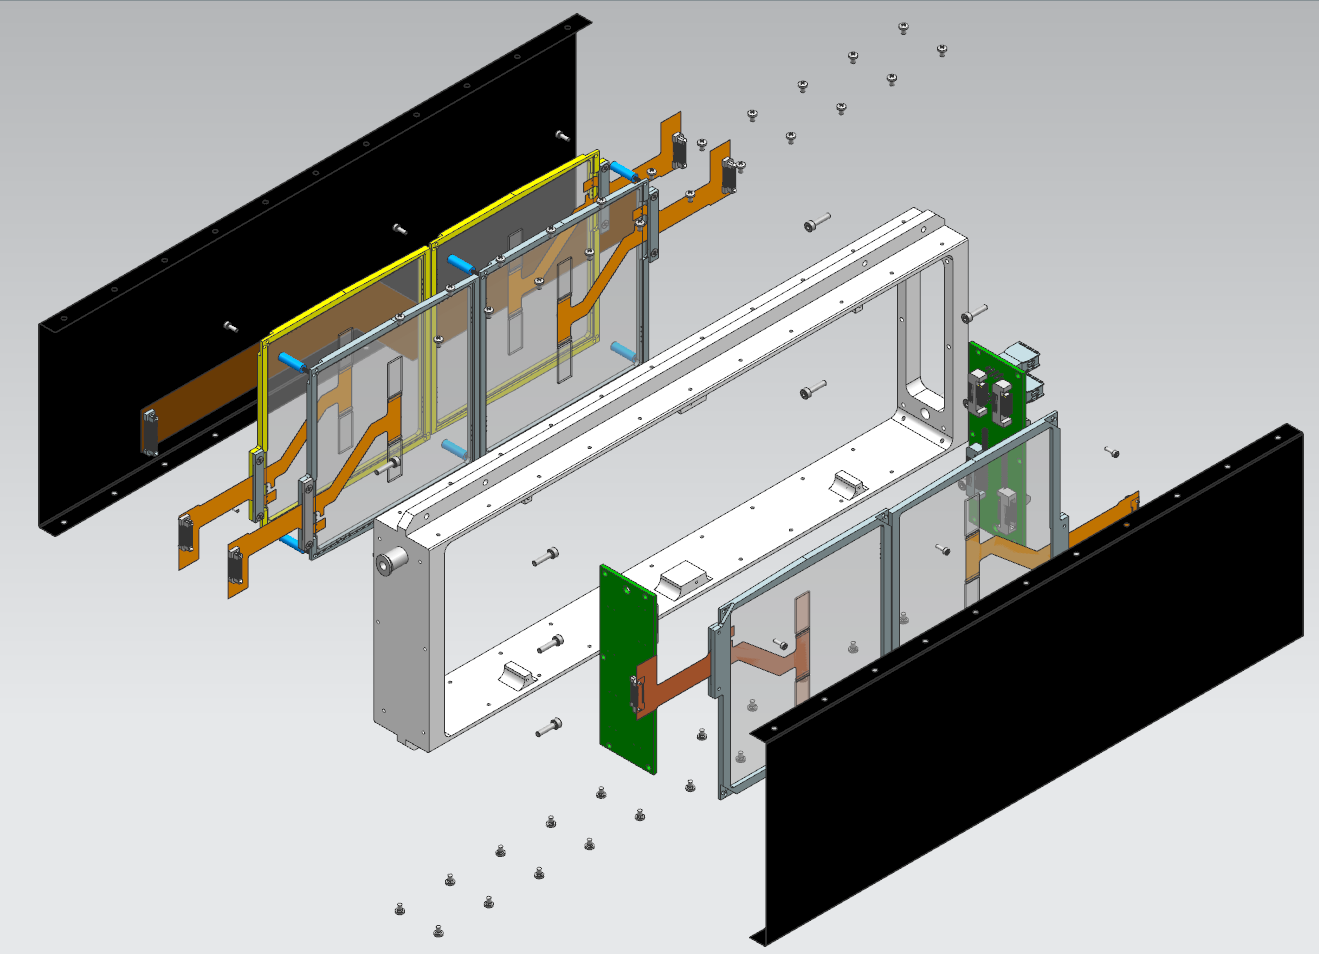
\includegraphics[width=0.8\linewidth]{pics/Explosion.png}
\caption{CAD drawing of each component of one half of the telescope,
i.e. 3 layers of two micro-strip sensors in parallel,
installed in a cassette-like support with 2 local readout electronic support at the endplate.}
\label{fig:intro1}
\end{figure}

\subsection{SiD Hybrid-less Micro-Strip Sensor}

%The 10$\times$\SI{10}{\square\centi\metre} SiD tracker strip sensor at a pitch of \SI{25}{\micro\metre}, readout by two 1024-channel ASICs, KPiX~\cite{kpix}, can provide a resolution of around \SI{7.2}{\micro\metre},
%was hence chosen, and the other requirements can be achieved by a \SI{2}{\degree} tilt. This sensor was originally developed for the SiD Detector Concept for the ILC~\cite{Behnke:2013lya}.
\begin{figure}[!t]
\centering
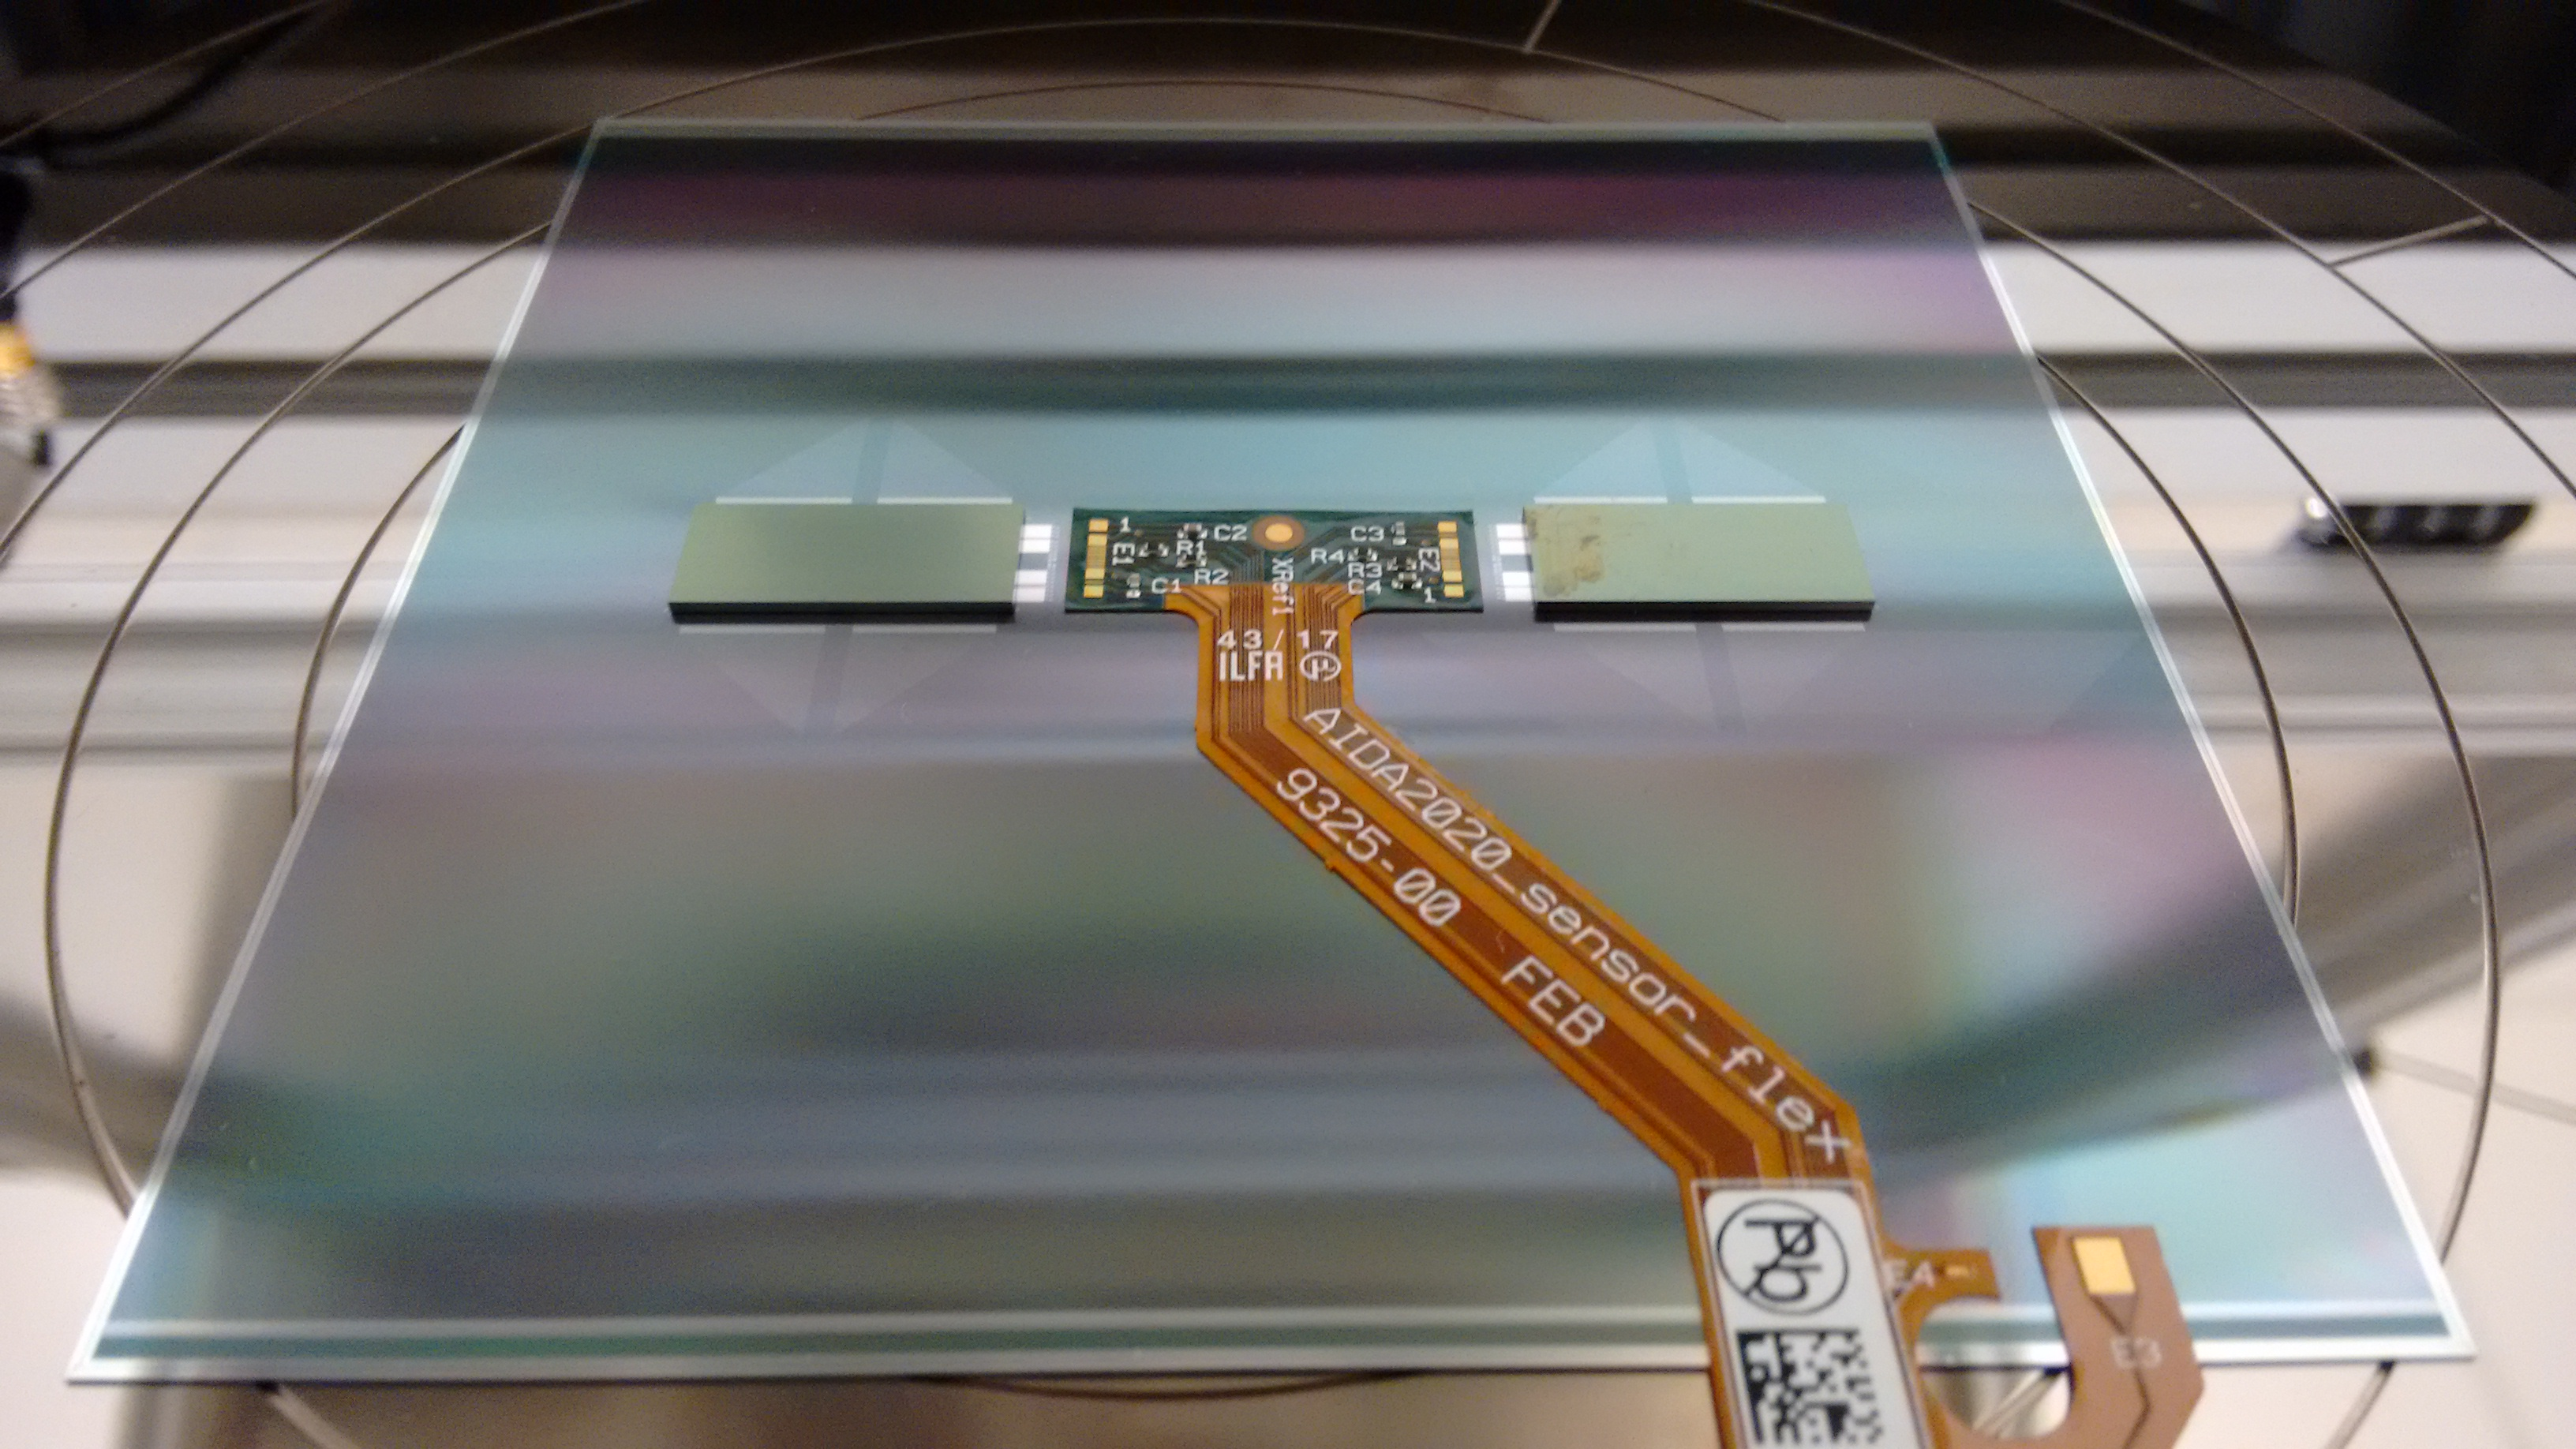
\includegraphics[width=2.5in]{pics/sensor_module1.jpg}
\caption{photo of an assembled module with two bump-bonded KPiX chips.
A kpaton flex cable is glued on the sensor,
and communicate with the KPiX through a second metallization layer.}
\label{fig:sensor}
\end{figure}

The SiD strip sensor is readout by a bump-bonded 1024-channel ASIC, KPiX, through a second metallization layer.
KPiX digitize the signal with a 13 bit ADC resolution, then send it out through one single data trace rounted on the second metallization layer to a wirebonded kapton cable, see Fig.~\ref{fig:sensor}.
This hybrid-less organizing eliminates the complex with the tranditional hybrid method, and it is the first time verified / tested on this micro-strip sensor.

The KPiX chip runs in a pulse cycle mode with a time resolution based on a \SI{100}{MHz} clock, and it can record up to four events per cycle for each channel.
The KPiX readout system was characterized before the strip sensor produced with several hexagonal pixel sensors, which were originally designed for the SiD ECAL~\cite{Behnke:2013lya}.
This ECal sensor was later used as a reference device in the testbeam for the strip sensor.
%These tests included understanding how to synchronize the KPiX chip data taking cycles to the DESY beam structure, as well as to other devices, like the TLU, and various DUTs.
%It was tested first with a $^{90}$Sr source in the lab, and then in the DESY test beam with energies from 4 to \SI{6}{\GeV} in May and October 2017~\cite{lycoris1}.

The strip sensors were delivered by Hamamatsu in summer 2017, showing very good electric features and all fully depleted at around \SI{50}{\volt}, see Figure~\ref{fig:2}.
% The first assembled sensors, see one example in Figure~\ref{fig:1figs} (right), were tested in spring 2018, with a $^{90}$Sr source in the lab at DESY, and several DESY test beam weeks are in schedule in fall 2018.
% Figure~\ref{fig:2figs} (right) shows the fired strip distribution over one data taking run, collected by one KPiX chip in a self-trigger mode from one assembled module, using a $^{90}$Sr source ,
% demonstrating that the assembled module is capable of seeing signals.
The first assembled sensors were produced early spring 2018, then examined firstly in the lab, then moved to the DESY-II Testbream Facility for testing in the summer 2018.

\begin{figure}[!ht]%
  \centering
  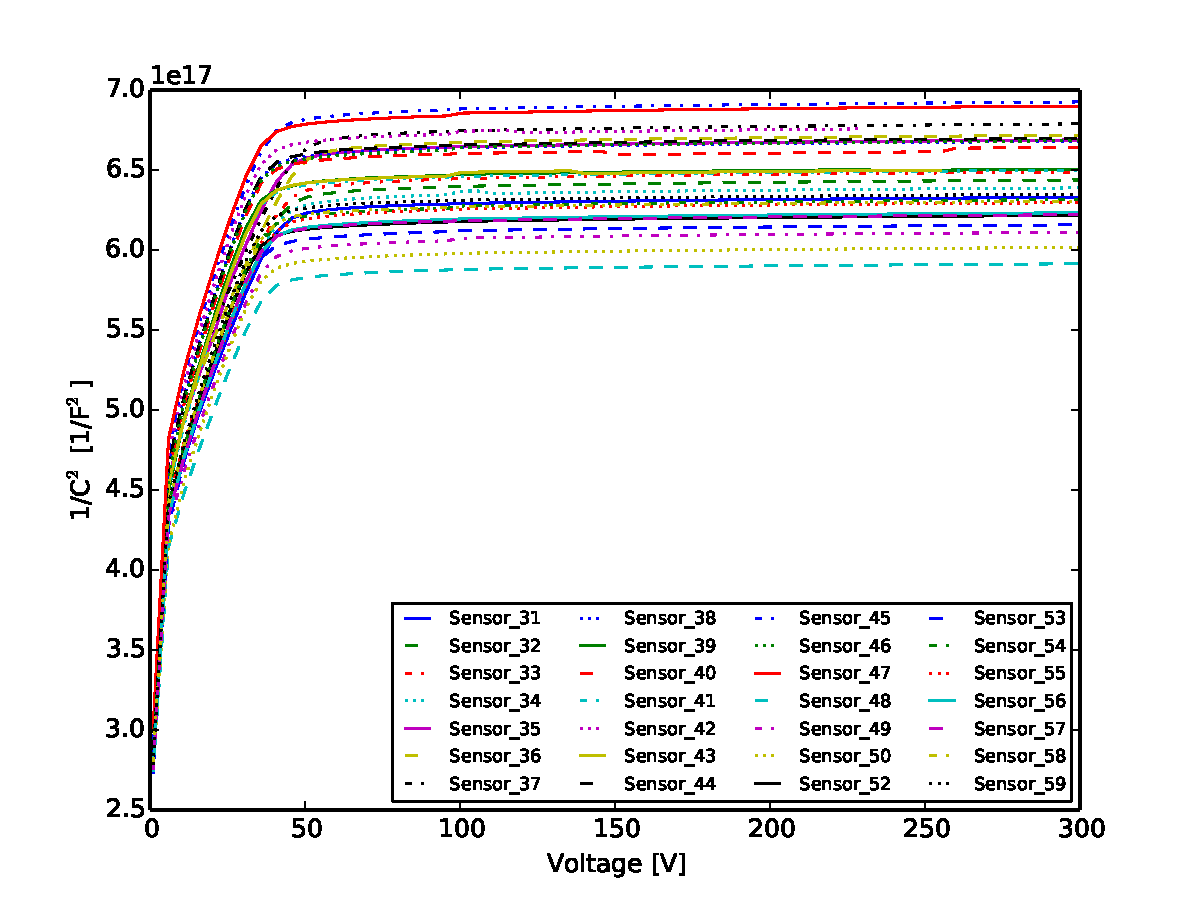
\includegraphics[width=1.0\linewidth]{pics/All_sensors_CV.pdf}
  \caption{C-V curves measured on all the bare sensors delivered from Hamamatsu in summer 2017, indicating all the sensors starts to be fully depleted, at around \SI{50}{\volt}.}%
\label{fig:2}%
\end{figure}


\section{Lab Test}
The test setup holding structure is grounded as a Faraday shield to provide a relative clean environment.
Temperary adapter used instead of the final electronic system, therefore cables are lying around the sensor under test inside the sheild, which is expected to pollute the signal.
Various data taking mode were tested in the lab, including ADC over Charge response calibration, forced trigger pedestal measurement, self-trigger mode run with background noise and with signal.
\begin{figure}[!ht]%
  \centering
  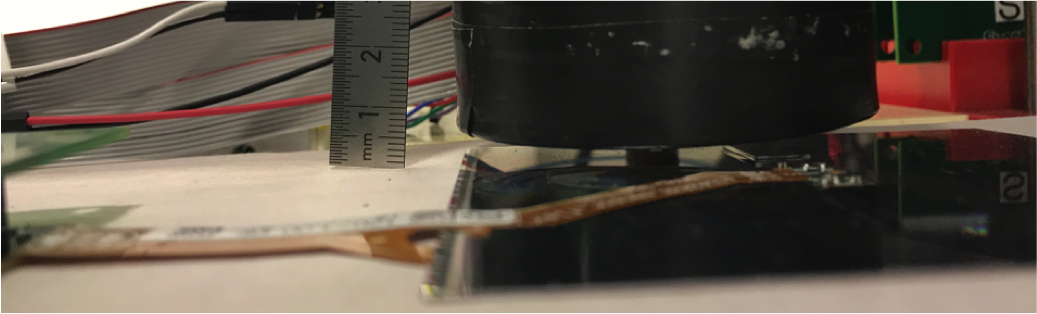
\includegraphics[width=1.0\linewidth]{pics/lab_1.png}
  \caption{ $^90Sr$ radioactive source point at the sensor closely with a collimator, in the lab.}%
\label{fig:lab1}%
\end{figure}

A preliminary noise level of ~0.5fC is determined from the forced trigger pedestal measurement, see the blue line distribution in Figure~\ref{}.
%The external trigger run mode can only be tested efficiently in the test beam because the $^{90}Sr$ is largely decreased after passing through the scintillator or through the sensor.
Under the self-trigger mode, various run configuration were tested, including threshold scan to chose one threshold with background triggered events largely suppressed.
$^{90}Sr$ source was used for signal runs, and the sensor is able to locate the signal position, as seen in Figure~\ref{fig:lab2} (right).
\begin{figure}[!ht]%
  \centering
  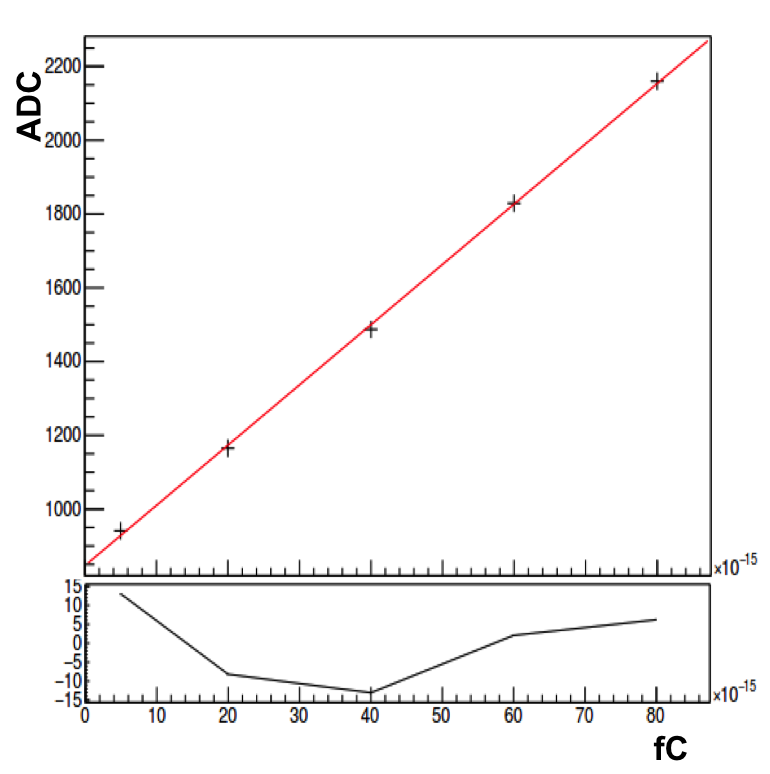
\includegraphics[width=0.4\linewidth]{pics/lab_2.png}%
  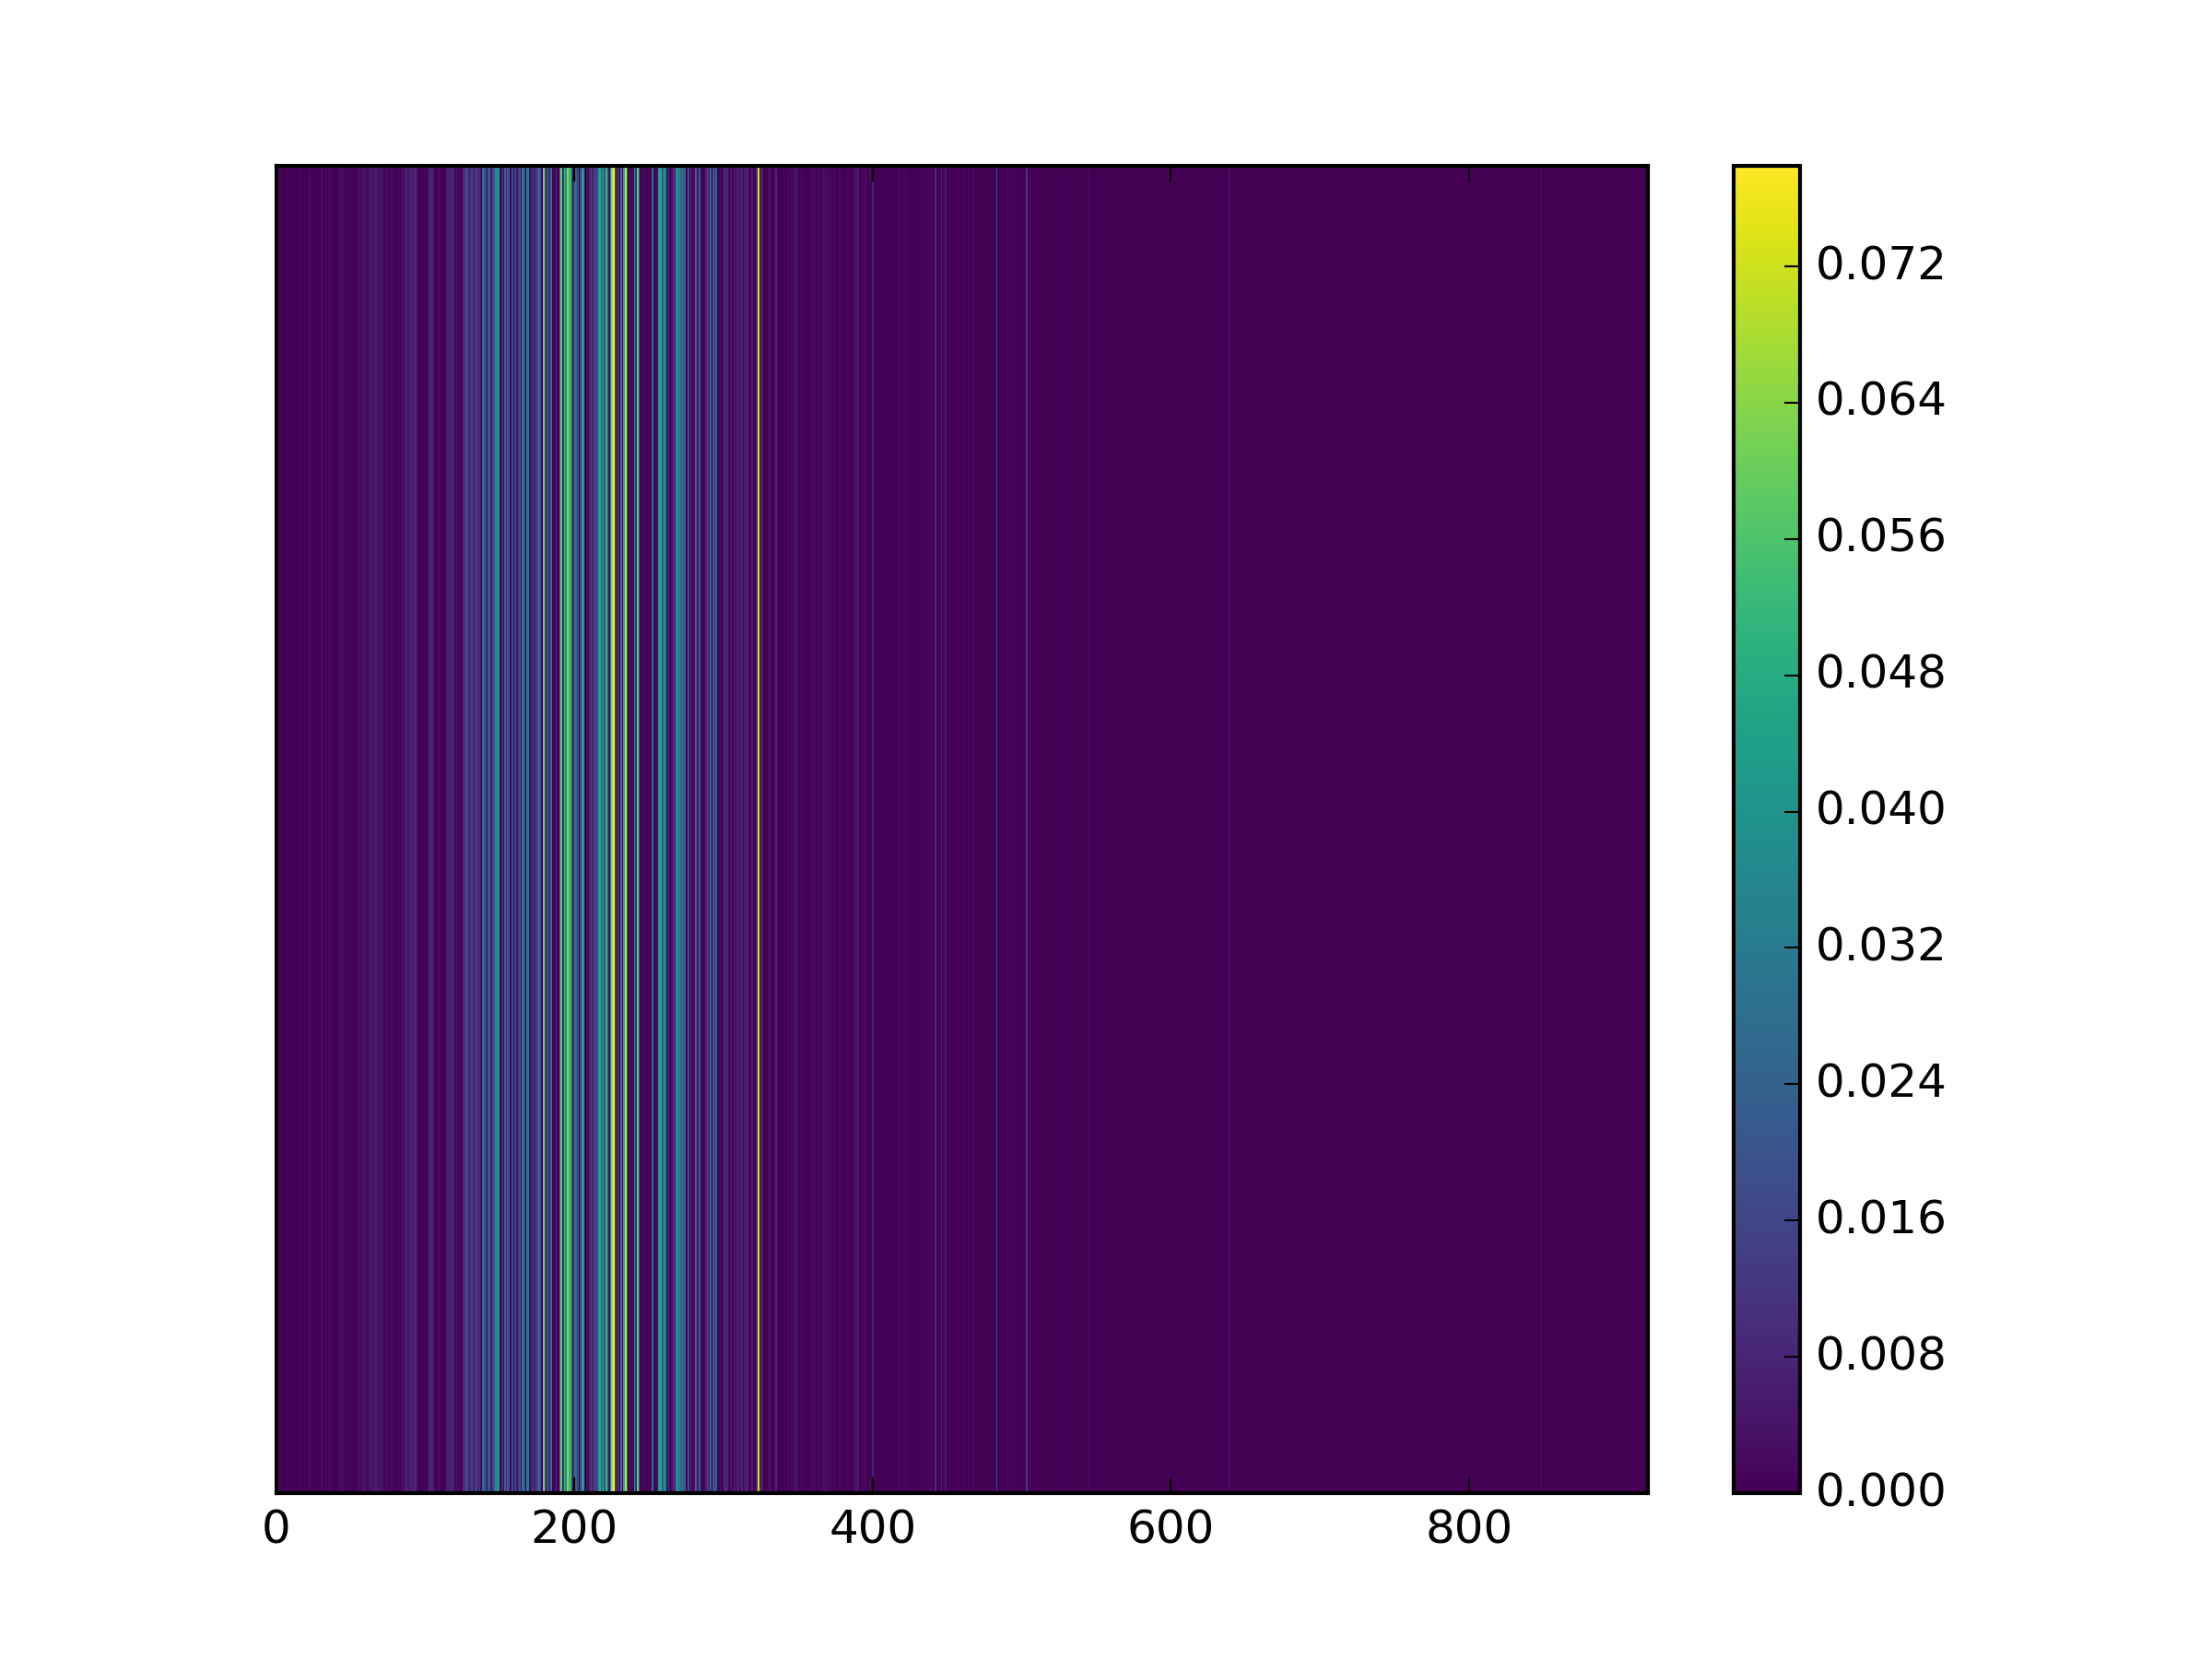
\includegraphics[width=0.6\linewidth]{pics/2018_07_13_16_34_20_strip_map_left.png}
  \caption{
  left: the upper plot shows fC vs ADC from calibration data and a linear fit (red) is drawn to determine the slope, the corresponding residual plot is shown in the lower pad;
  right: the x-axis illustrates all the strips on the left side of the sensor, z-axis shows the possibility to register one event per acquisition cycle.
  }%
\label{fig:lab2}%
\end{figure}


\section{Test Beam}
The DESY-II test beam area T24/1 was used, its infrastructure description see~\cite{desytbf}.
The beam energy was chosen to be 3GeV in order to get the best beam rate, and a $9\times9 mm^2$ secondary collimator was chosen
It turns out to be 5kHz trigger rate over the device active time, the beam collimator was chosen to be
The test setup at the test beam is similar to the one in the lab, but the following differences were applied.
1) Sensors were held in the final support, a grounded cassette, see photo~\ref{fig:tb2}.
2) A hexagonal pixel sensor plane was placed beneath the micro-strip sensor as a reference device, which employs the same kpix chip and the same readout system.
3) Two scintillators installed right after the secondary collimator, before the micro-strip sensor, which were connected to a series of NIM modules to provide a conincidence to the kpix readout system.

\begin{figure}[!ht]%
  \centering
  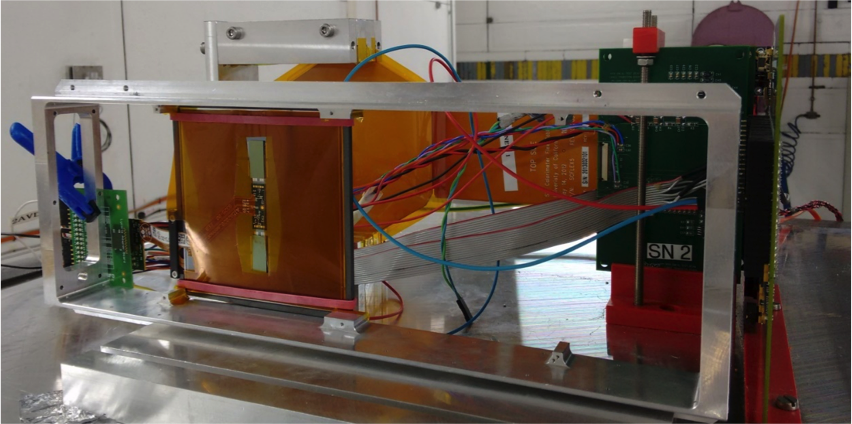
\includegraphics[width=1.0\linewidth]{pics/tb_2.png}
  \caption{Test beam setup.}%
\label{fig:tb2}%
\end{figure}

\begin{figure}[!ht]%
  \centering
  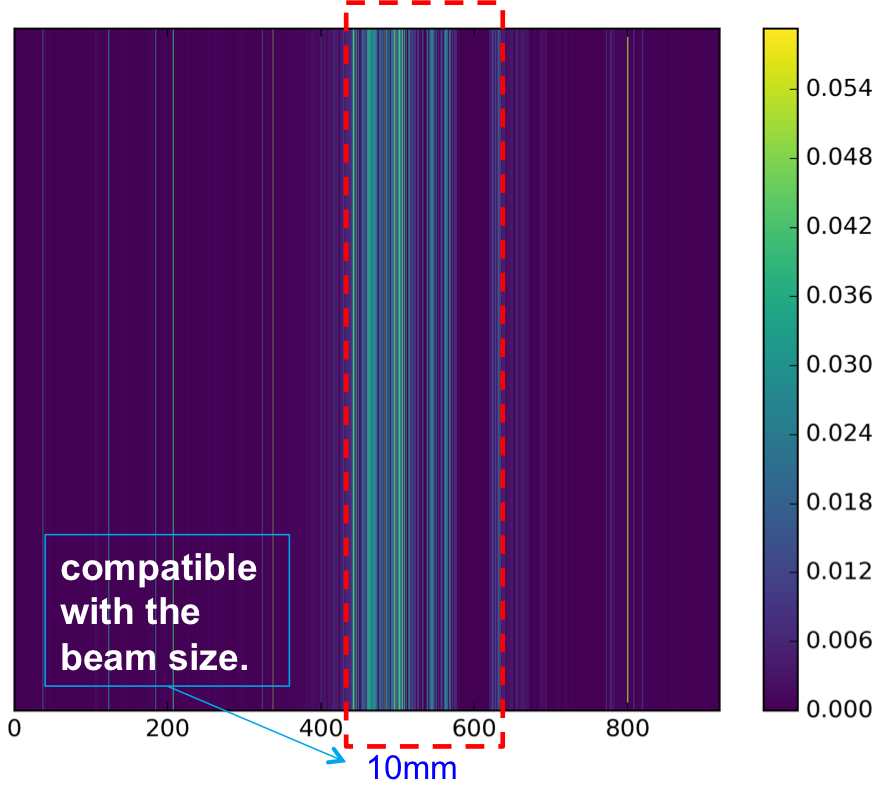
\includegraphics[width=0.8\linewidth]{pics/tb_1.png}
  \caption{Test beam setup.}%
\label{fig:tb1}%
\end{figure}

\subsection{Results and Discussion}

Self-trigger mode, with external trigger time stamps, one can plot the time difference between self-triggers and external triggers, in order to study the time features of an event, see Fig.~\ref{fig:res1}.
Two clear bump can be seen every minimum trigger time unit (8 times BunchClockCount is the reset time after a trigger), which comes from events retriggered from closing neighbour channels.
This can be used in the future as a cut to clean such events.
\begin{figure}[!ht]%
  \centering
  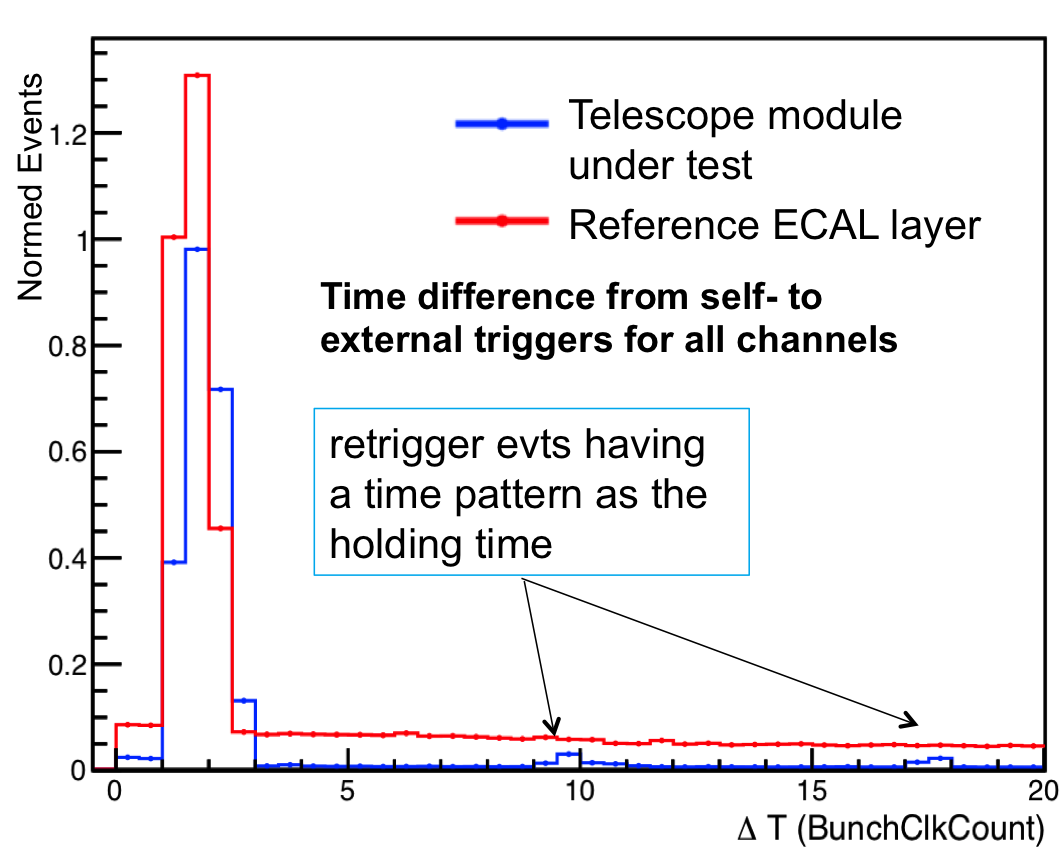
\includegraphics[width=1.0\linewidth]{pics/Res_pic1.png}
  \caption{Self-trigger mode}%
\label{fig:res1}%
\end{figure}

Self-trigger mode, with a relative low threshold and external trigger time stamps.
Events which can be correlated to an external trigger time stamp, is shown in Fig.~\ref{fig:res2}.
The time correlated events very well replicate the tail of the all events ditribution on ADC, and it can even be fit with a naive Landau fit, see the small plot on Fig.~\ref{fig:res2}.

\begin{figure}[!ht]%
  \centering
  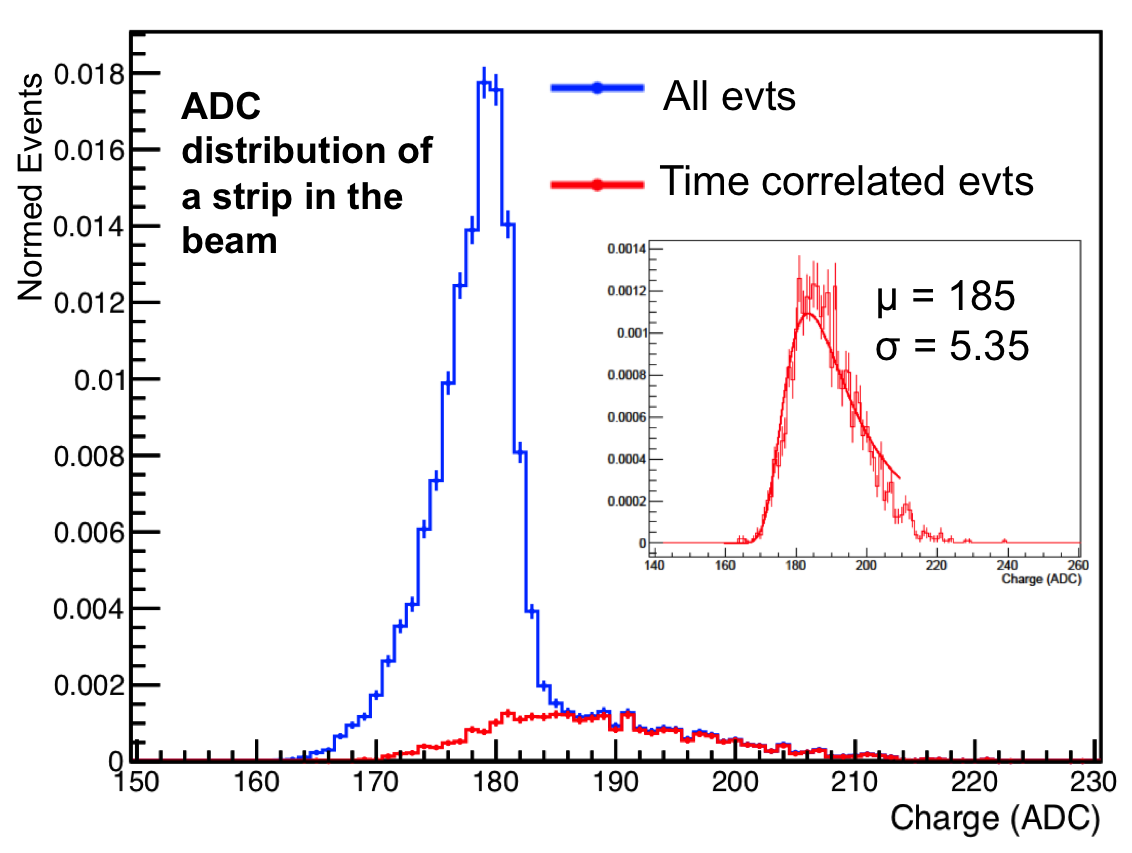
\includegraphics[width=1.0\linewidth]{pics/Res_pic2.png}
  \caption{Self-trigger mode}%
\label{fig:res2}%
\end{figure}

This time correlated study was carried out on data with various different threshold, to purify the self-triggered events, see Fig.~\ref{fig:res3}.

\begin{figure}[!ht]%
  \centering
  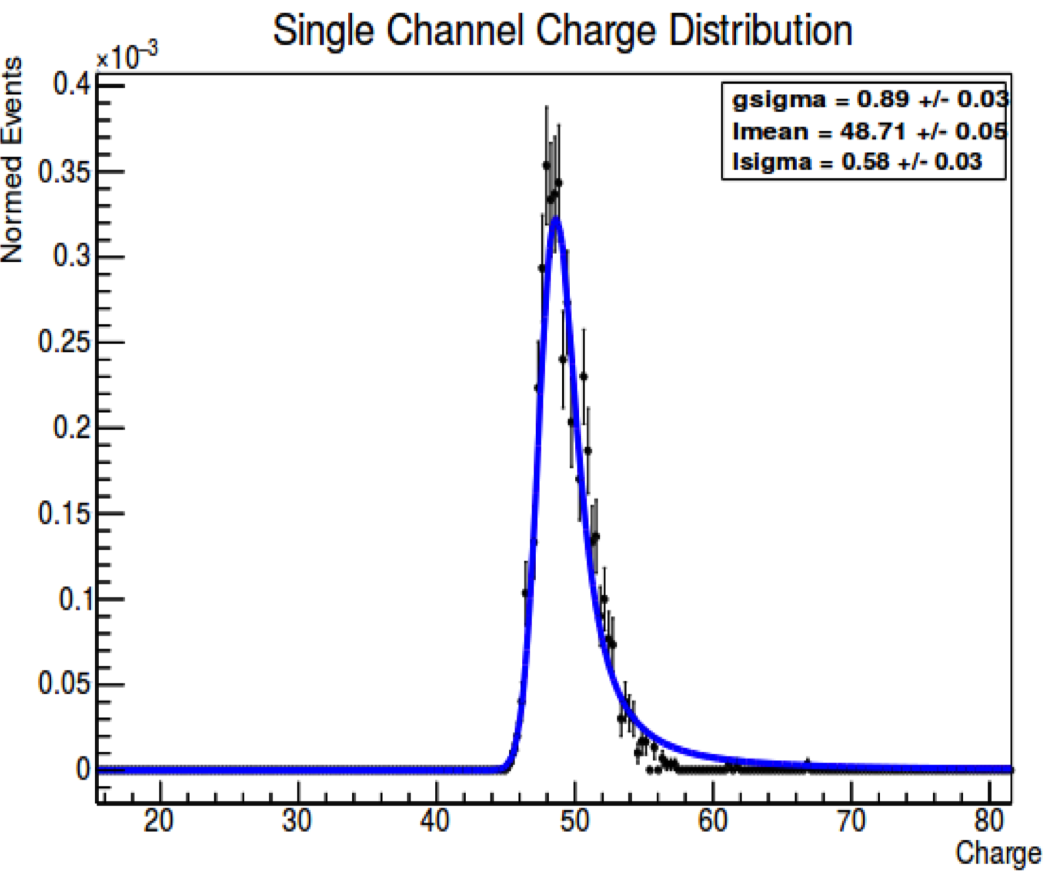
\includegraphics[width=1.0\linewidth]{pics/Res_pic3.png}
  \caption{Self-trigger mode}%
\label{fig:res3}%
\end{figure}

All the results shown here are without pedestal subtraction, due to a known issue of the pedestal shifting due to power cycling.

%%%%%%%----------------------

% An example of a floating figure using the graphicx package.
% Note that \label must occur AFTER (or within) \caption.
% For figures, \caption should occur after the \includegraphics.
% Note that IEEEtran v1.7 and later has special internal code that
% is designed to preserve the operation of \label within \caption
% even when the captionsoff option is in effect. However, because
% of issues like this, it may be the safest practice to put all your
% \label just after \caption rather than within \caption{}.
%
% Reminder: the "draftcls" or "draftclsnofoot", not "draft", class
% option should be used if it is desired that the figures are to be
% displayed while in draft mode.
%
%\begin{figure}[!t]
%\centering
%\includegraphics[width=2.5in]{myfigure}
% where an .eps filename suffix will be assumed under latex,
% and a .pdf suffix will be assumed for pdflatex; or what has been declared
% via \DeclareGraphicsExtensions.
%\caption{Simulation results for the network.}
%\label{fig_sim}
%\end{figure}

% Note that the IEEE typically puts floats only at the top, even when this
% results in a large percentage of a column being occupied by floats.


% An example of a double column floating figure using two subfigures.
% (The subfig.sty package must be loaded for this to work.)
% The subfigure \label commands are set within each subfloat command,
% and the \label for the overall figure must come after \caption.
% \hfil is used as a separator to get equal spacing.
% Watch out that the combined width of all the subfigures on a
% line do not exceed the text width or a line break will occur.
%
%\begin{figure*}[!t]
%\centering
%\subfloat[Case I]{\includegraphics[width=2.5in]{box}%
%\label{fig_first_case}}
%\hfil
%\subfloat[Case II]{\includegraphics[width=2.5in]{box}%
%\label{fig_second_case}}
%\caption{Simulation results for the network.}
%\label{fig_sim}
%\end{figure*}
%
% Note that often IEEE papers with subfigures do not employ subfigure
% captions (using the optional argument to \subfloat[]), but instead will
% reference/describe all of them (a), (b), etc., within the main caption.
% Be aware that for subfig.sty to generate the (a), (b), etc., subfigure
% labels, the optional argument to \subfloat must be present. If a
% subcaption is not desired, just leave its contents blank,
% e.g., \subfloat[].


% An example of a floating table. Note that, for IEEE style tables, the
% \caption command should come BEFORE the table and, given that table
% captions serve much like titles, are usually capitalized except for words
% such as a, an, and, as, at, but, by, for, in, nor, of, on, or, the, to
% and up, which are usually not capitalized unless they are the first or
% last word of the caption. Table text will default to \footnotesize as
% the IEEE normally uses this smaller font for tables.
% The \label must come after \caption as always.
%
%\begin{table}[!t]
%% increase table row spacing, adjust to taste
%\renewcommand{\arraystretch}{1.3}
% if using array.sty, it might be a good idea to tweak the value of
% \extrarowheight as needed to properly center the text within the cells
%\caption{An Example of a Table}
%\label{table_example}
%\centering
%% Some packages, such as MDW tools, offer better commands for making tables
%% than the plain LaTeX2e tabular which is used here.
%\begin{tabular}{|c||c|}
%\hline
%One & Two\\
%\hline
%Three & Four\\
%\hline
%\end{tabular}
%\end{table}


% Note that the IEEE does not put floats in the very first column
% - or typically anywhere on the first page for that matter. Also,
% in-text middle ("here") positioning is typically not used, but it
% is allowed and encouraged for Computer Society conferences (but
% not Computer Society journals). Most IEEE journals/conferences use
% top floats exclusively.
% Note that, LaTeX2e, unlike IEEE journals/conferences, places
% footnotes above bottom floats. This can be corrected via the
% \fnbelowfloat command of the stfloats package.


\section{Conclusion}
% The \lycoris telescope is scheduled to be delivered early 2019, with a TLU and a reconstruction software ready-to-use for user.
% In this contribution, the \lycoris telescope will be presented, with its first results and a comparison to simulation;
% the characterization of the sensor and readout system will also be included.

This is the first application of the SiD hybrid-less micro-strip sensor, from which the sensor with its featured readout system are characterized systematically.
The very first assembled modules were examined with various run conditions in the lab, and the following features are verified:
1) 80-85\% readout channels shown good ADC to charge reponse, as well as relatively low noise (0.5 fC);
2) sensor is able to see signal out of noise under self-trigger mode, and locate the signal position.

The first beam test result not only confirms what has been verified in the lab, but also shows a lower noise (0.2 fC) with the sensor better shielded with the final support structure.
The external trigger run mode is first studied on this sensor at the test beam, the result is not shown in this contribution but it turns out to give promising signal to background ratio after pedestal subtraction.
signal efficiency is also firstly be tested under self-trigger mode with a timing conincidence to the external trigger,


% conference papers do not normally have an appendix


% use section* for acknowledgment
\section*{Acknowledgment}


The authors would like to thank ...


This project has received funding from the European Union’s Horizon 2020 Research and Innovation programme under Grant Agreement no. 654168.


% trigger a \newpage just before the given reference
% number - used to balance the columns on the last page
% adjust value as needed - may need to be readjusted if
% the document is modified later
%\IEEEtriggeratref{8}
% The "triggered" command can be changed if desired:
%\IEEEtriggercmd{\enlargethispage{-5in}}

% references section

% can use a bibliography generated by BibTeX as a .bbl file
% BibTeX documentation can be easily obtained at:
% http://mirror.ctan.org/biblio/bibtex/contrib/doc/
% The IEEEtran BibTeX style support page is at:
% http://www.michaelshell.org/tex/ieeetran/bibtex/
%\bibliographystyle{IEEEtran}
% argument is your BibTeX string definitions and bibliography database(s)
%\bibliography{IEEEabrv,../bib/paper}
%
% <OR> manually copy in the resultant .bbl file
% set second argument of \begin to the number of references
% (used to reserve space for the reference number labels box)
\begin{thebibliography}{1}

%\bibitem{IEEEhowto:kopka}
%H.~Kopka and P.~W. Daly, \emph{A Guide to \LaTeX}, 3rd~ed.\hskip 1em plus
% 0.5em minus 0.4em\relax Harlow, England: Addison-Wesley, 1999.

\bibitem{aida2020}
AIDA2020 homepage \url{http://aida2020.web.cern.ch}, accessed on 2018-04-05.

\bibitem{desytbf}
DESY II Test Beam Facility \url{http://testbeam.desy.de}, accessed on 2018-04-05.

\bibitem{eudet}
H.~Jansen et al., {\em Performance of the EUDET-type beam telescopes}, \textbf{EPJ Tech.\ Instrum.\  {\bf 3}, no. 1, 7 (2016)}.

\bibitem{kpix}
J.~Brau et al., {\em KPiX - A 1,024 channel readout ASIC for the ILC}, \textbf{in 2012 IEEE Nuclear Science Symposium and Medical Imaging Conference Record (NSS/MIC), pp. 1857–1860, Oct 2012.}.

\bibitem{Behnke:2013lya}
T.~Behnke et al.,{\em The International Linear Collider Technical Design Report - Volume 4: Detectors}  \textbf{arXiv:1306.6329 [physics.ins-det]}

\bibitem{eudaq2}
Y.~Liu., {\em EUDAQ2 User Manual}, \textbf{AIDA-2020-NOTE-2018-001}.

\bibitem{lycoris1}
U.~Kraemer et al., {\em LYCORIS - A Large Area Strip Telescope}, \textbf{arXiv:1801.08505 [physics.ins-det]}.

\end{thebibliography}




% that's all folks
\end{document}
